\documentclass[11pt]{article}

% Page layout and typography
\usepackage[margin=1in]{geometry}
\usepackage[T1]{fontenc}
\usepackage{lmodern}
\usepackage{microtype}

% Scientific writing
\usepackage{amsmath,amssymb}
\usepackage{graphicx}
\usepackage{booktabs}
\usepackage{tabularx}
\usepackage{cite}

% Links and references
\usepackage[hidelinks]{hyperref}

\title{Single-LLM Versus Multi-Agent Debate Systems for Scientific Hypothesis Generation}
\author{
  \parbox{0.9\textwidth}{\centering
    \mbox{}\\
    Department of Information Technology, Indian Institute of Information Technology Allahabad, Uttar Pradesh, India
  }
}
\date{}

\begin{document}

\maketitle

\begin{abstract}
Large language models (LLMs) are increasingly being used to propose scientific hypotheses,
retrieve and synthesize literature, critique candidate explanations, and support experimental design.
Two broad paradigms have emerged: single-LLM systems that rely on one model with prompting,
retrieval, self-reflection, or tool use; and multi-agent systems in which several model instances
interact through debate, role specialization, iterative review, or consensus formation. This review
compares these paradigms for scientific hypothesis generation. Rather than treating multi-agent
interaction as automatically superior, the literature is organized around five themes: hypothesis
generation and novelty, evidence grounding and verification, critique and debate, evaluation of
scientific quality, and integration with autonomous research workflows. The reviewed studies
suggest that single-LLM systems offer simplicity, lower cost, easier control, and strong
performance when supplied with suitable literature or domain tools. Multi-agent systems can
improve exploration, criticism, and the explicit comparison of competing ideas, particularly when
agents are genuinely diverse and are assigned complementary roles. However, debate introduces
substantial costs and can amplify shared model errors, sycophancy, premature consensus, and
problem drift. The strongest direction is therefore not a binary choice but a conditional hybrid
architecture: independent generation followed by evidence retrieval, targeted adversarial review,
selective debate, and experimental validation. Important gaps remain in standardized benchmarks,
causal attribution of multi-agent gains, calibration, diversity measurement, and real-world
laboratory validation.
\end{abstract}

\noindent\textbf{Keywords:} large language models; scientific hypothesis generation; multi-agent systems; debate;
literature-based discovery; autonomous science; evaluation

\section{Introduction}
\label{sec:introduction}

Scientific discovery depends on the ability to connect observations, identify regularities, formulate explanatory hypotheses, and determine which hypotheses deserve empirical testing. Computational approaches to discovery have a long history. Early systems such as BACON, a computational scientific-discovery system designed to identify regularities in observed data and formulate candidate scientific laws, demonstrated that programs could search observations for regularities and express them as candidate scientific laws, while literature-based discovery showed that useful knowledge can emerge by connecting information that is distributed across otherwise separate bodies of research \cite{swanson1986undiscovered,langley1987scientific}.

Recent LLMs have changed the scale and flexibility of this problem. Instead of relying only on manually designed discovery rules, an LLM can summarize literature, propose mechanisms, combine concepts, generate experiments, and revise ideas in natural language. Studies have examined both direct hypothesis generation \cite{zhou2024hypothesis,yang2024large} and broader research automation, including literature retrieval, coding, experimentation, and manuscript preparation \cite{lu2024ai,yamada2026towards}. A single-LLM approach can also provide a relatively simple and lower-cost way of supporting scientific reasoning, functioning as an accessible assistant that can generate and refine ideas without requiring the coordination of multiple agents.

At the same time, researchers have begun to replace the single model with groups of interacting agents. In these systems, one agent may generate ideas, another may act as a critic, and others may assess novelty, feasibility, evidence, or experimental design. Multi-agent debate is attractive because scientific reasoning is not only a process of generating explanations; it is also a process of challenging them. Multiple agents can introduce different perspectives and provide repeated opportunities for critique and refinement. However, this interaction increases computational and engineering costs and may also produce agreement without correctness, particularly when agents share similar biases or reinforce unsupported claims.

These trade-offs suggest that the comparison need not be limited to choosing between a single LLM and a fully multi-agent system. The lower cost and simplicity of single-LLM approaches and the diversity and critical evaluation offered by multi-agent systems could potentially be combined or selectively optimized. A hybrid approach could therefore use the appropriate level of interaction depending on the scientific task, research question, or stage of hypothesis generation. The central question is therefore not simply whether multiple agents outperform one, but under what conditions different combinations of single-LLM and multi-agent capabilities are most suitable for scientific hypothesis generation.

This review addresses that question through the following research question: \textbf{How do single-LLM and multi-agent debate systems differ in their ability to generate novel, valid, feasible, and experimentally useful scientific hypotheses, and what design choices determine their relative advantages?} The review focuses on systems that produce scientific ideas or hypotheses, while also considering adjacent work on reasoning, self-reflection, scientific agents, and automated experimentation.



\subsection{Scientific hypothesis generation with LLMs}
\label{subsec:hypothesis-generation}

A scientific hypothesis can be viewed as a structured, testable proposition that links observations,
variables, mechanisms, or interventions. In practical research, a useful hypothesis must satisfy
several conditions at once: it should be sufficiently novel, connected to existing evidence,
scientifically plausible, operationally testable, and potentially consequential. These criteria can
conflict. An idea that is highly novel may be weakly grounded; an idea that is strongly supported by
existing literature may be incremental.

Computational discovery systems traditionally separated the search for candidate regularities from
the evaluation of those candidates. BACON-like systems searched data for patterns and formulated
laws \cite{langley1987scientific}. Literature-based discovery approaches instead searched textual or
bibliographic spaces for meaningful connections \cite{swanson1986undiscovered}. LLM-based
systems combine aspects of these functions through a flexible language interface, but their
hypothesis-generation mechanism is fundamentally different from conventional rule-based
discovery.

An LLM generates text by estimating a probability distribution over possible next tokens
conditioned on the preceding context. In simplified form, the probability of a generated sequence
can be expressed as
\begin{equation}
P(y_{1:T}\mid x)=\prod_{t=1}^{T}P(y_t\mid y_{<t},x),
\end{equation}
where $x$ denotes the input context, $y_t$ is the token generated at position $t$, and
$y_{<t}$ represents the preceding generated tokens. Consequently, hypothesis generation does not
require the model to explicitly discover a scientific law or perform a formally valid inference.
Instead, the model can generate candidate explanations by recombining patterns and relationships
represented in its learned parameters and the supplied context.

This raises an important question: is probabilistic text generation scientifically sound as a basis
for hypothesis generation? The answer depends on what is meant by ``sound.'' Probabilistic
generation by itself does not establish that a hypothesis is scientifically true, causally valid, or
even factually correct. A highly probable continuation may simply reflect patterns frequently
present in the training data. LLMs can therefore produce hypotheses that are plausible in language
while being unsupported by evidence. This limitation is particularly important because the
probability assigned to a generated sequence should not be interpreted as a probability that the
scientific hypothesis itself is true.

However, scientific hypothesis generation is inherently exploratory. A hypothesis is a proposition
to be tested rather than a conclusion that is already known to be correct. Recent work therefore
argues that the probabilistic and sometimes unexpected outputs of LLMs can be useful for proposing
candidate hypotheses, provided that those candidates are subsequently evaluated using scientific
evidence or experiments. Zhou et al. demonstrate that LLM-generated hypotheses can be iteratively
updated from observed data and can improve predictive performance over simple few-shot prompting
in several benchmark settings \cite{zhou2024hypothesis}. Laboratory validation provides stronger
evidence for the feasibility of this approach: GPT-4 generated candidate drug combinations, several
of which subsequently showed positive experimental synergy, although the study also reported
limitations in the quality of the explanations accompanying the generated hypotheses
\cite{abdelrehim2025scientific}.

Thus, the scientific value of an LLM-generated hypothesis should not be judged from the generation
probability alone. The LLM can be viewed as a mechanism for exploring a large space of candidate
ideas, while novelty, evidential grounding, plausibility, feasibility, and experimental validity
must be assessed separately. This distinction is central to comparing single-LLM systems with
multi-agent approaches: the main question is not which architecture generates the most plausible
text, but which architecture more reliably converts generated candidates into scientifically useful
hypotheses.

\subsection{Single-LLM systems}
\label{subsec:single-llm}

A single-LLM system uses one model instance as the principal generator and reasoner. It may be
enhanced through prompt engineering, chain-of-thought-style reasoning, retrieval-augmented
generation, external tools, memory, self-critique, or iterative refinement. Self-Refine and Reflexion
illustrate the broader idea that a single model can generate an output, inspect it, and revise it using
feedback or memory \cite{madaan2023selfrefine,shinn2023reflexion}.

The single-LLM paradigm should therefore not be equated with a single prompt. A single model
can perform multiple stages internally or sequentially. The defining feature is that the stages are
controlled by one model rather than by independently instantiated agents with potentially different
roles or instructions.

\subsection{Multi-agent debate systems}
\label{subsec:multi-agent}

Multi-agent systems distribute the process across several model instances or agent roles. A typical
workflow includes independent proposal, critique, rebuttal, synthesis, and ranking. Debate may be
open-ended, role-based, or mediated by a coordinator. The motivation is to increase search breadth
and create explicit disagreement before a final decision.

Multi-agent debate was initially studied for factuality and reasoning rather than scientific ideation
specifically. Du et al. reported that debate can improve performance on some reasoning and
factuality tasks \cite{du2024improving}. However, later analysis showed that multi-agent debate does
not reliably dominate simpler baselines and is sensitive to configuration, cost, and task
characteristics \cite{smit2024mad}. These findings are directly relevant to scientific hypothesis
generation, where the quality of the evaluation process may matter more than the number of agents.

\section{Thematic Literature Review}
\label{sec:thematic-literature-review}

\subsection{Theme 1: Generation, novelty, and exploration}
\label{subsec:generation-novelty-exploration}

One major contribution of LLMs is their ability to generate candidate research directions from large
amounts of scientific language. Zhou et al. study hypothesis generation with LLMs and show how
prompting and data-driven formulations can be used to produce candidate hypotheses
\cite{zhou2024hypothesis}. Yang et al. similarly investigate automated open-domain scientific
hypothesis discovery, demonstrating the potential of LLMs to move beyond narrow question
answering toward research-oriented generation \cite{yang2024large}.

However, novelty is difficult to define and measure. A generated statement may be linguistically
unusual while being scientifically trivial, already known, or impossible to test. SciMON (Scientific
Inspiration Machines for Optimizing Novelty) addresses this issue by retrieving scientific inspirations
and optimizing candidate ideas for novelty \cite{wang2024scimon}. Its design implies that novelty
should be treated as a search objective informed by literature, not as a property inferred only from
the wording of the output.

Human evaluation studies reinforce this distinction. Si et al. evaluate LLM-generated research ideas
with a large group of NLP researchers and examine dimensions such as novelty and feasibility
\cite{si2025novel}. Their work suggests that LLMs can produce ideas that are competitive in some
respects, but it also shows why expert assessment remains necessary: research quality involves
implicit disciplinary knowledge and judgments about whether an idea would actually advance the
field.

Multi-agent systems potentially improve exploration by allowing several agents to propose
alternatives before synthesis. Su et al. report that a multi-agent scientific-ideation system can
improve idea quality relative to single-agent baselines under their evaluation protocol
\cite{su2025many}. The likely mechanism is not merely parallel text generation. Different agents
can search different conceptual paths, expose assumptions, and preserve alternatives that a single
generation might discard too early.

Nevertheless, more agents do not automatically imply more useful diversity. If all agents share the
same model, prompts, retrieval corpus, and priors, their proposals may be highly correlated.
Diversity must therefore be designed through independent sampling, role variation, different
evidence views, or explicit disagreement objectives.

\subsection{Theme 2: Evidence grounding, literature retrieval, and verification}
\label{subsec:evidence-grounding}

Scientific hypotheses cannot be evaluated solely by fluency. They must be connected to
observations, prior findings, mechanisms, and feasible measurements. Literature grounding is
consequently central to both single- and multi-agent systems. Zhou et al. emphasize the importance
of using scientific data and context in hypothesis generation \cite{zhou2024hypothesis}, while
SciMON explicitly retrieves literature-based inspirations to guide novelty \cite{wang2024scimon}.

Evidence grounding can improve factuality and reduce the risk that an LLM invents unsupported
mechanisms. It also makes the generated hypothesis more useful to researchers because the system
can identify supporting findings, conflicting evidence, and missing experiments. However, retrieval
alone does not guarantee correctness. A model may misinterpret a paper, cite evidence that does not
entail the claim, or combine results from incompatible settings.

The distinction between single-LLM and multi-agent approaches is therefore not necessarily a
distinction between what a model can and cannot do. A single LLM can be organized into sequential
stages in which it retrieves evidence, generates a hypothesis, critiques the proposal, and revises
it. Multi-agent architectures make these roles explicit by assigning them to separate interacting
agents. Such separation can provide specialized prompts, independent critiques, different contexts,
or parallel reasoning paths, but it also introduces additional computational and coordination costs.
The potential advantage of multi-agent systems therefore depends on whether these additional
sources of diversity and specialization improve the evaluation process beyond what can be achieved
through sequential use of a single model.

The AI co-scientist line of work illustrates a broader generate--debate--evolve pattern, where
candidate ideas are repeatedly assessed and refined \cite{gottweis2025towards}. The Virtual Lab
similarly demonstrates the value of connecting agentic reasoning to experimental validation rather
than treating textual agreement as the final endpoint \cite{virtuallab2024}. These approaches do
not necessarily imply that multiple agents are always required; rather, they illustrate how
structured interaction and iterative evaluation can be incorporated into scientific discovery.

Both approaches can also inherit the same fundamental evidence-related limitations. If the initial
retrieval is incomplete, a single-LLM pipeline or every downstream agent may reason over the same
missing evidence. Likewise, additional agents may multiply rather than correct errors if they rely
on the same unsupported information. A robust architecture should therefore record provenance,
distinguish retrieved evidence from model inference, and require explicit statements of uncertainty.


\subsection{Theme 3: Critique, self-reflection, and debate}
\label{subsec:critique-debate}

Critique is the strongest conceptual argument for multi-agent debate. Scientific reasoning requires
identifying hidden assumptions, alternative explanations, confounding variables, and weaknesses in
experimental design. Single-LLM systems can perform self-critique through iterative prompting.
Self-Refine uses feedback-driven revision \cite{madaan2023selfrefine}, and Reflexion adds verbal
feedback and memory to support future attempts \cite{shinn2023reflexion}. These methods can be
effective when the model is capable of recognizing its own errors.

However, self-critique is not independent criticism. The same model that generated a hypothesis
also supplies the criteria, interpretation, and final judgment. It may rationalize its first answer
instead of genuinely challenging it. Multi-agent debate addresses this problem by separating
proposal and criticism across agents. Du et al. provide general evidence that debate can improve
some reasoning and factuality outcomes \cite{du2024improving}.

Scientific ideation introduces additional complexity. Debate participants may disagree about
novelty, feasibility, or importance even when they agree on the underlying facts. Smit et al. caution
that multi-agent debate is not universally better than self-consistency or ensembling and that
performance depends on the debate strategy and task \cite{smit2024mad}. This is especially
important for scientific hypotheses because there is often no immediate ground-truth answer.

Debate can also create undesirable social dynamics among agents. Agents may converge on an early
proposal because it is repeated frequently, appears authoritative, or is presented with high
confidence. Consensus can therefore be a poor proxy for scientific validity. The most useful debate
design is likely adversarial but structured: agents should be required to state evidence, identify
falsification conditions, propose alternatives, and preserve unresolved disagreement.

\subsection{Theme 4: Evaluation of scientific quality}
\label{subsec:evaluation-quality}

Evaluation remains the central bottleneck in the literature. Common dimensions include novelty,
relevance, significance, feasibility, validity, clarity, and potential impact. These dimensions are
related but not interchangeable. A hypothesis can be novel but implausible, feasible but
unimportant, or significant but already established.

IdeaBench proposes a benchmark-oriented approach to research-idea generation and emphasizes
systematic evaluation of research ideas \cite{guo2025ideabench}. The biomedical evaluation by Qi
et al. similarly considers multiple dimensions, including novelty, relevance, significance, and
verifiability \cite{qi2024biomedical}. Such work is important because it moves evaluation away
from a single LLM-judge score.

Experimental validation provides a stronger form of evidence. Boiko et al. demonstrate autonomous
chemical research with LLMs, showing how language-based reasoning can be connected to
laboratory procedures \cite{boiko2023autonomous}. The breast-cancer laboratory study provides
another example of LLM-generated drug-combination hypotheses being tested experimentally
\cite{scientific2025laboratory}. These studies do not establish that one architecture is universally
superior, but they show that scientific usefulness ultimately depends on whether generated ideas
survive contact with experiments.

Multi-agent systems may improve evaluation by assigning separate agents to novelty, feasibility,
evidence, and risk. However, this decomposition can create false precision. Scores from several
agents may look rigorous while still reflecting the same model biases. Evaluation should therefore include external evidence, expert judgment, prospective prediction, and where possible, experimental success.
These evaluation challenges become particularly important as hypothesis generation is incorporated into broader autonomous research workflows.

\subsection{Theme 5: From hypothesis generation to autonomous science}

The literature increasingly treats hypothesis generation as one stage in an end-to-end research loop.
The AI Scientist attempts to automate idea generation, coding, experimentation, analysis, and paper
writing \cite{lu2024ai}. The AI co-scientist and related systems extend this idea through multiple
agents, iterative debate, and evidence-based evolution \cite{gottweis2025towards}.

These systems suggest that the single-versus-multi distinction is becoming less clear in practice. A
single agent may call tools and perform multiple internal roles, while a multi-agent system may use
a coordinator that effectively behaves like a single decision-maker. The more useful comparison is
therefore functional: how many independent searches occur, how criticism is generated, how
evidence is checked, and how final decisions are validated.

End-to-end automation also exposes limitations. Autonomous systems may generate
underdeveloped ideas, implement experiments incorrectly, or produce manuscripts that appear
coherent despite methodological weaknesses \cite{lu2024ai,yamada2026towards}. This reinforces
the need for human oversight and explicit validation gates.

\section{Comparison of Existing Approaches}
\label{sec:comparison}

Single-LLM and multi-agent systems should be compared across several dimensions rather than by
one overall score. Table~\ref{tab:system-comparison} summarizes the main differences identified in
the literature across cost, search breadth, criticism, evidence use, reproducibility, scalability, and
validation.

\begin{table}[htbp]
  \centering
  \caption{Comparison of single-LLM and multi-agent systems for scientific hypothesis generation.}
  \label{tab:system-comparison}
  \small
  \renewcommand{\arraystretch}{1.2}
  \begin{tabularx}{\textwidth}{@{}>{\raggedright\arraybackslash}p{0.18\textwidth}
                                  >{\raggedright\arraybackslash}X
                                  >{\raggedright\arraybackslash}X@{}}
    \toprule
    \textbf{Dimension} & \textbf{Single-LLM Systems} & \textbf{Multi-Agent Systems} \\
    \midrule
    Cost and efficiency & Lower computational and orchestration cost
                        & Higher token use, latency, and coordination cost \\
    Search breadth      & Multiple samples possible through prompting
                        & Explicit parallel exploration of diverse ideas \\
    Criticism           & Self-reflection and internal critique
                        & Independent, role-based criticism and debate \\
    Evidence use        & Single evidence path; simpler pipeline
                        & Evidence work can be distributed across agents \\
    Reproducibility     & Easier to reproduce
                        & Depends on agent roles, topology, and debate configuration \\
    Scalability         & Scales through model and tool improvements
                        & Scales through additional agents, with coordination costs \\
    Validation          & Requires external experimental validation
                        & Also requires external experimental validation \\
    \bottomrule
  \end{tabularx}
\end{table}

\begin{itemize}
  \item \textbf{Cost and efficiency.} Single-LLM systems generally require fewer model calls and are
  easier to deploy. Multi-agent debate increases token use, latency, orchestration complexity, and
  often the number of retrieval operations.

  \item \textbf{Search breadth.} A single model can generate multiple samples, but multi-agent systems
  make parallel exploration explicit. Their advantage depends on whether agents are genuinely
  diverse.

  \item \textbf{Criticism.} Self-reflection is cheap and easy to integrate, but multi-agent criticism can
  provide more independent perspectives. Neither guarantees correctness.

  \item \textbf{Evidence use.} Both paradigms benefit from retrieval and tools. Multi-agent systems can
  divide evidence work, but shared retrieval errors may propagate across agents.

  \item \textbf{Reproducibility.} Single-LLM pipelines are easier to specify and reproduce. Multi-agent
  results depend on agent roles, communication topology, stopping rules, and debate order.

  \item \textbf{Scalability.} Single-LLM systems scale through larger models, better prompts, and tools.
  Multi-agent systems scale through additional agents, but coordination costs and convergence
  problems may increase.

  \item \textbf{Validation.} Neither architecture is sufficient without external checks. Laboratory or
  prospective validation is stronger than textual consensus.
\end{itemize}

Overall, the literature does not support a universal claim that multi-agent debate is superior.
Multi-agent systems appear most useful when the task benefits from independent search, specialized
criticism, or explicit comparison of competing hypotheses. Single-LLM systems remain attractive
when cost, speed, reproducibility, and strong tool integration are more important.These differences become clearer when the systems are decomposed by function rather than treated as indivisible architectures.

\subsection{A functional comparison of system components}
\label{subsec:functional-comparison}

Both paradigms may contain generation, retrieval, critique, ranking, memory, and tool use.
The difference lies in how these functions are allocated.
In a single-LLM pipeline, one model usually performs several functions sequentially or through structured
prompting. In a multi-agent pipeline, the functions are distributed across model instances that
communicate through messages or shared artifacts. Consequently, the number of agents alone is not
a sufficient measure of architectural sophistication. Figure~\ref{fig:functional-allocation} visualizes
this functional allocation, showing how the same broad activities can be organized within a
single-LLM pipeline or distributed across specialized agents.

\begin{figure}[htbp]
  \centering
  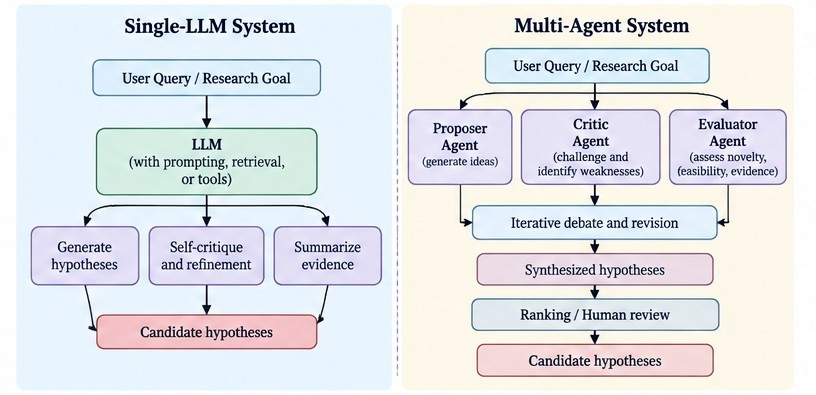
\includegraphics[width=\textwidth]{figures/functional-comparison.jpg}
  \caption{Conceptual comparison of single-LLM and multi-agent systems for scientific hypothesis generation. Single-LLM systems rely on one model with prompting, retrieval or tool use, while multi-agent systems employ specialized agents that interact through debate, critique and iterative revision to produce and refine candidate hypotheses.}
  \label{fig:functional-allocation}
\end{figure}

The first functional component is candidate generation. A single model can generate multiple
candidates through temperature sampling, prompt variation, or repeated calls. This may
approximate a population of agents, but the candidates are often produced under highly similar
assumptions. Multi-agent systems can make independence explicit by assigning different agents
different starting points, disciplinary perspectives, or evidence subsets. The benefit is greatest when
the agents are encouraged to preserve competing explanations rather than immediately optimize for
consensus.

The second component is evaluation. A single-LLM system can ask the model to score novelty,
plausibility, and feasibility, but the scores may be internally correlated with the original generation.
In a multi-agent system, separate critics can be instructed to challenge different dimensions. For
example, one critic can focus on whether the claim follows from the literature, another can inspect
the proposed mechanism, and a third can design a falsification test. This decomposition may
improve coverage, but it also creates an aggregation problem: a final controller must decide how to
combine disagreement without reducing all judgments to a superficial average.

The third component is evidence management. Retrieval-augmented generation, citation tracing,
structured notes, and tool calls can be used in either paradigm. A single-LLM system is often easier
to audit because the evidence path is shorter. A multi-agent system can distribute retrieval and
verification, but it must maintain provenance across agents. Without a shared record of which paper
supports which statement, the system may produce a polished synthesis whose evidential basis is
difficult to inspect.

\subsection{Why more agents may help---and why they may not}
\label{subsec:more-agents}

The potential advantage of multiple agents can be understood partly as a reduction in the risk of
shared reasoning failures. If agents independently approach a problem, disagreement may reveal an
overlooked assumption or an alternative mechanism. This is particularly valuable in open-ended
science, where there is rarely a single immediately verifiable answer. However, independence is a
design property, not an automatic consequence of using multiple model instances. Agents sharing the
same model, prompt template, retrieved papers, and evaluation rubric may reproduce the same error
several times. Recent work on multi-agent debate also shows that agents can reinforce one another
and converge on incorrect conclusions rather than correcting them \cite{pitre2025consensagent}.

There is also a distinction between productive disagreement and noisy disagreement. Productive
disagreement is specific: an agent identifies a missing control, questions a causal interpretation,
or proposes a test that could distinguish two mechanisms. Noisy disagreement merely produces
different wording or unsupported objections. Studies of multi-agent research dialogues suggest that
agent diversity and interaction depth can affect the quality and diversity of generated ideas, but
these factors do not necessarily improve every aspect of the resulting output
\cite{ueda2025design}. A useful debate protocol should therefore require each critique to identify
the exact claim being challenged, the evidence or assumption involved, and the consequence for the
proposed experiment. This makes the debate more auditable and reduces the risk that verbosity is
mistaken for reasoning quality.

Another limitation is premature convergence. Once one hypothesis is presented confidently or
repeated by several agents, later agents may treat it as the default and modify it only superficially.
Such convergence can be efficient when the leading hypothesis is correct, but dangerous when the
initial proposal is flawed. Evidence of consensus and sycophantic agreement in multi-agent debate
suggests that additional agents do not automatically provide independent validation
\cite{pitre2025consensagent}. Scientific systems should therefore preserve a small number of serious
alternatives until evidence-based ranking or experimental testing provides a reason to eliminate
them.

\subsection{The role of human researchers in the comparison}
\label{subsec:human-researchers}

The single-versus-multi-agent comparison should not be framed as a replacement contest between
models and scientists. Human researchers contribute domain knowledge, tacit standards of
evidence, awareness of practical constraints, and judgment about which questions matter. These
contributions are difficult to capture fully in automated scores. In a single-LLM workflow, the
researcher may guide the prompt, select sources, and inspect the generated hypothesis. In a
multi-agent workflow, the researcher may additionally design roles, set debate rules, resolve
disagreements, and approve experiments.

Human involvement is especially important at the transition from textual plausibility to scientific
action. A hypothesis may be interesting but require unavailable equipment, an ethically
unacceptable experiment, an unmeasured confounder, or a sample size that makes the proposed test
impractical. A human-in-the-loop design can use LLMs for breadth and structured criticism while
retaining human authority over interpretation, safety, and experimental prioritization. This
arrangement also creates a more realistic evaluation target: the value of a system may be measured
by how much it improves a scientist's decisions, not only by the quality of its standalone text.

\section{Research Trends and Developments}
\label{sec:research-trends}

\begin{enumerate}
  \item \textbf{Literature-grounded generation.} Systems increasingly retrieve papers, extract evidence,
  and use scientific knowledge to constrain generation
  \cite{zhou2024hypothesis,wang2024scimon,qi2024biomedical}.

  \item \textbf{Agent specialization.} Multi-agent systems assign roles such as generator, critic,
  literature analyst, experimental designer, and risk assessor
  \cite{su2025many,gottweis2025towards}.

  \item \textbf{Closed-loop discovery.} Research systems increasingly connect hypothesis generation
  with coding, experiments, analysis, and revision
  \cite{lu2024ai,yamada2026towards,gottweis2025towards,boiko2023autonomous}.

  \item \textbf{Benchmarking and structured evaluation.} Recent work emphasizes novelty, feasibility,
  validity, verifiability, and impact rather than fluency alone
  \cite{si2025novel,guo2025ideabench,qi2024biomedical}.

  \item \textbf{Experimental validation.} Laboratory studies are beginning to test whether LLM-generated
  ideas produce measurable scientific value
  \cite{virtuallab2024,boiko2023autonomous,scientific2025laboratory}.

  \item \textbf{Risk-aware scientific agents.} As systems become more autonomous, safety, citation
  faithfulness, uncertainty, and human oversight become central design requirements
  \cite{goo2026citation,safescientist2025,hong2024metagpt}.
\end{enumerate}

\subsection{A proposed evaluation framework}
\label{subsec:evaluation-framework}

A rigorous comparison should evaluate the complete hypothesis-generation process. The first
dimension is novelty, measured against a time-stamped literature corpus and supplemented by
expert judgment. The second is scientific validity, including whether the hypothesis is consistent
with known observations and whether its causal or mechanistic explanation is coherent. The third is
feasibility, which includes the availability of data, instruments, samples, and realistic experimental
procedures. The fourth is predictive value: a strong hypothesis should make a sufficiently specific
prediction that could be checked later.

The fifth dimension is diversity. Systems should be evaluated not only on the best idea they produce
but also on the range of mechanisms and experimental directions they explore. A set of ten
paraphrases should not count as ten independent discoveries. The sixth dimension is calibration:
confidence should track the strength of the evidence. The seventh is efficiency, including token use,
number of model calls, latency, retrieval cost, and human review time. Reporting these dimensions
together would prevent a system from appearing superior merely because it uses substantially more
computation.

A useful experimental design would include at least four matched conditions: a single LLM with
one generation, a single LLM with multiple sampled candidates, a multi-agent system without
debate, and a multi-agent system with structured debate. All conditions should receive the same
model family, literature access, token budget where possible, and evaluation instructions. This
design would help determine whether any observed improvement comes from agent interaction
itself or simply from generating more candidates.

Evaluation should also separate retrospective and prospective settings. In retrospective evaluation,
the system is given a known literature corpus and its outputs are compared with existing findings.
This is useful for testing grounding and rediscovery, but it may reward ideas that are already
implicit in the data. In prospective evaluation, hypotheses are generated before a later result is
known and are scored against subsequent experiments or publications. Prospective evaluation is
more difficult, but it better measures whether a system contributes to actual discovery.

\section{Challenges and Limitations}
\label{sec:challenges-limitations}

Scientific novelty is difficult to operationalize. Similarity-based measures may reward unusual
wording, whereas expert ratings can be subjective and expensive. Scientific validity often cannot
be determined from the existing literature alone; it requires experiments or prospective prediction.
LLMs may also hallucinate mechanisms, references, or experimental outcomes. These risks are
especially serious when a multi-agent system repeats and reinforces an unsupported claim.

Multi-agent debate also incurs substantial engineering costs. Its performance depends on the
number of agents, role prompts, communication structure, debate rounds, and aggregation method
\cite{smit2024mad}. Consensus may suppress minority ideas, and agents may converge prematurely
on a plausible but incorrect explanation. Moreover, many evaluations rely on LLM judges, which
can introduce shared biases and make systems appear stronger than they are.

Finally, the available evidence is heterogeneous: studies use different domains, prompts, models,
datasets, expert panels, and evaluation scales. Results from biomedical hypothesis generation
therefore cannot automatically be generalized to chemistry, materials science, social science, or
theoretical research. Comparisons between single- and multi-agent systems are also often
confounded by unequal token budgets, retrieval access, or model capability.

\subsection{Reproducibility and reporting requirements}
\label{subsec:reproducibility}

Future studies should report sufficient implementation detail to enable meaningful comparisons.
Required details include the exact model and version, prompts, temperature and sampling settings,
retrieval corpus and cutoff date, number of agents, role descriptions, communication topology,
number of debate rounds, stopping criteria, judge prompts, and total token expenditure. Without
these details, an apparent advantage may result from hidden differences in compute or information
access.

Researchers should also report negative results and failure cases, including duplicated hypotheses,
unsupported citations, incorrect interpretations of papers, unresolved disagreement, and
experiments that fail because the proposed mechanism was not operationalized correctly. Such
reporting is particularly important for scientific applications because a system may appear
successful under language-based evaluation yet fail when its claims are tested in the laboratory.

\section{Research Gaps}
\label{sec:research-gaps}

\begin{enumerate}
  \setcounter{enumi}{6}
  \item \textbf{Controlled architecture comparisons.} Studies should compare single- and multi-agent
  systems with matched models, token budgets, retrieval access, and tool permissions.

  \item \textbf{Causal analysis of debate.} Experiments should isolate whether gains come from parallel
  sampling, role specialization, critique, additional computation, or simply more generated text.

  \item \textbf{Better diversity metrics.} Research needs measures of conceptual diversity that distinguish
  genuinely different mechanisms from paraphrases.

  \item \textbf{Calibration and uncertainty.} Systems should report confidence, evidence strength,
  disagreement, and conditions under which a hypothesis would be falsified.

  \item \textbf{Prospective and experimental validation.} Benchmarks should track whether hypotheses
  lead to successful future predictions or laboratory results.

  \item \textbf{Domain-sensitive evaluation.} Different fields require different definitions of novelty,
  feasibility, evidence, and significance.

  \item \textbf{Failure-mode reporting.} Papers should report hallucinations, unsupported citations,
  duplicated ideas, premature consensus, and failed experiments rather than only average scores.

  \item \textbf{Human--AI collaboration.} More work is needed on when scientists should intervene, how
  they should inspect agent reasoning, and how human expertise changes the quality of the final
  hypothesis.
\end{enumerate}

\subsection{Toward adaptive debate}
\label{subsec:adaptive-debate}

An especially promising direction is adaptive debate rather than mandatory debate. Most candidate
hypotheses may not require a large agent discussion. A lightweight single-LLM pass could first
generate and filter candidates. Only proposals with high potential impact, substantial disagreement,
weak evidence, or unusual safety concerns would be escalated to additional agents. This design
would preserve the main efficiency advantage of single-LLM systems while allocating multi-agent
computation where it is most likely to add value.

Adaptive systems could also vary the type of interaction. If the main uncertainty concerns novelty,
the system should retrieve and compare prior work. If the uncertainty concerns mechanism, it
should invoke a mechanistic critic. If the uncertainty concerns feasibility, it should ask an
experimental-design agent to specify controls, measurements, and failure conditions. In this way,
the architecture becomes evidence-driven rather than relying on a fixed number of agents or debate
rounds.

\section{Future Research Directions}
\label{sec:future-research}

A promising future architecture is a selective hybrid pipeline. First, several independent proposals
are generated, either by one model with controlled sampling or by multiple agents. Second, each
proposal is grounded in retrieved literature and linked to explicit evidence. Third, specialized critics
assess novelty, validity, feasibility, safety, and experimental design. Fourth, debate is activated only
for proposals with substantial disagreement or high potential value. Finally, a ranking model or
human researcher selects candidates for experimental testing. This proposed workflow is
summarized in Figure~\ref{fig:hybrid-workflow}.

\begin{figure}[htbp]
  \centering
  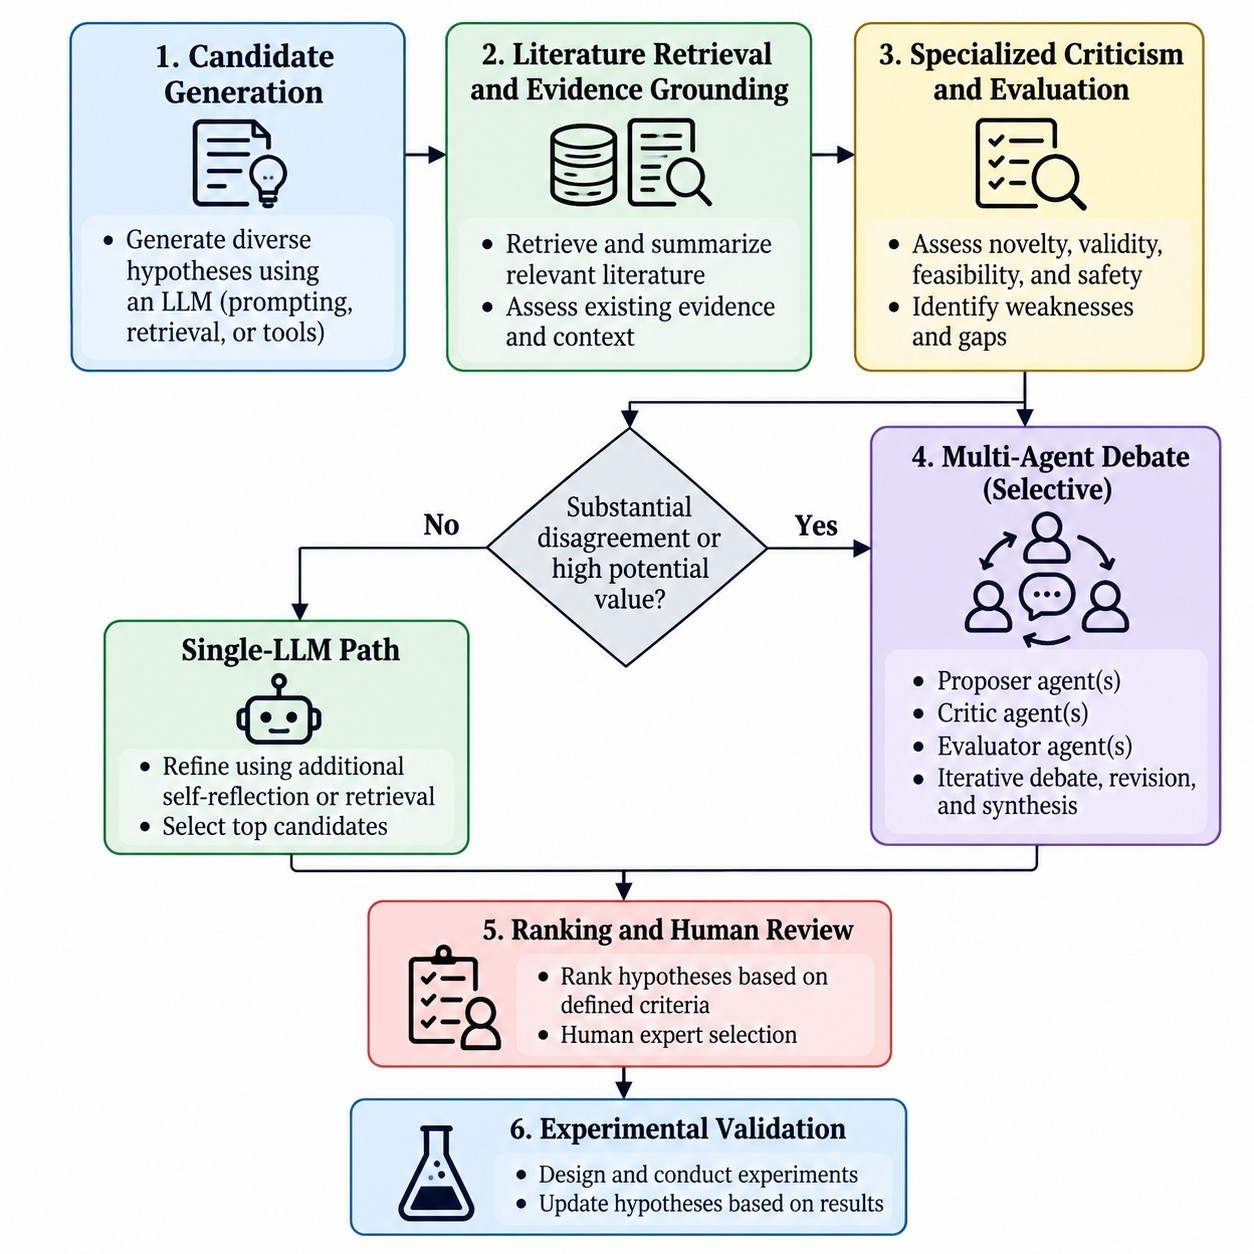
\includegraphics[width=0.9\textwidth]{figures/hybrid-workflow.jpg}
  \caption{Proposed hybrid workflow for scientific hypothesis generation. The system begins with candidate generation using a single LLM, followed by literature retrieval and specialized evaluation. Multi-agent debate is activated selectively when there is substantial disagreement among evaluators or high potential value in further exploration. The final candidates are ranked and reviewed by human experts before experimental validation.}
  \label{fig:hybrid-workflow}
\end{figure}

Future systems should preserve disagreement instead of forcing consensus. They should maintain
provenance graphs linking claims to papers, observations, assumptions, and proposed tests. They
should also use adaptive compute: easy cases can be handled by a single LLM, while difficult or
high-impact cases receive additional agents and verification.

Evaluation should move toward prospective benchmarks. A system should generate hypotheses
before a literature or experimental outcome is known, and later be scored on predictive success.
This would distinguish genuine discovery from retrospective repackaging. Finally, scientific agents
should be designed with risk-aware constraints, transparent uncertainty, and human approval before
consequential experiments.

\section{Conclusion}
\label{sec:conclusion}

Single-LLM and multi-agent debate systems represent complementary strategies for scientific
hypothesis generation. Single-LLM systems are efficient, reproducible, and increasingly capable
when combined with retrieval, self-reflection, and scientific tools. Multi-agent systems offer
explicit parallel exploration, role specialization, and criticism, but their benefits are conditional and
can be offset by cost, correlated errors, sycophancy, and premature consensus.

The literature therefore favors a conditional rather than universal conclusion. Multi-agent debate is
most valuable when it introduces meaningful independence, improves evidence checking, or
resolves substantive disagreement. Single-LLM systems may be preferable for rapid exploration,
constrained workflows, and applications where additional interaction does not improve validation.
In both cases, the decisive test is not fluent output or agent agreement, but whether a hypothesis is
novel, evidence-grounded, testable, and capable of producing useful scientific knowledge.

\nocite{*}
\bibliographystyle{unsrt}
\bibliography{references}

\end{document}
